\documentclass{acm_proc_article-sp}
\usepackage{graphicx}
\usepackage{balance}
\usepackage{fontspec}
\setmainfont[Ligatures={TeX}]{Times}
\usepackage{hyperref}
\graphicspath{{figures/}}

\hyphenation{metamarkets nelson}

\begin{document}

% ****************** TITLE ****************************************

\title{Druid: A Real-time Analytical Data Store}

% ****************** AUTHORS **************************************

\numberofauthors{6}
\author{
\alignauthor Fangjin Yang, Eric Tschetter, Gian Merlino, Nelson Ray, Xavier Léauté, Deep Ganguli, Himadri Singh\\
\email{\{fangjin, cheddar, gian, nelson, xavier, deep, himadri\}@metamarkets.com}
}
\date{21 March 2013}

\maketitle

\begin{abstract} 
Druid is an open
source\footnote{\href{https://github.com/metamx/druid}{https://github.com/metamx/druid}}
data store designed for real-time exploratory analytics on large data sets.
The system combines a column-oriented storage layout, a distributed,
shared-nothing architecture, and an advanced indexing structure to allow for
the arbitrary exploration of billion-row tables with sub-second latencies. In
this paper, we describe Druid's architecture, and detail how it supports fast
aggregations, flexible filters, and low latency data ingestion.  
\end{abstract}

\section{Introduction} 
In recent years, the proliferation of internet technology has
created a surge in machine-generated events.  Individually, these
events contain minimal useful information and are of low value.  Given the
time and resources required to extract meaning from large collections of
events, many companies were willing to discard this data instead.  Although
infrastructure has been built handle event based data (e.g. IBM's
Netezza\cite{singh2011introduction}, HP's Vertica\cite{bear2012vertica}, and EMC's
Greenplum\cite{miner2012unified}), they are largely sold at high price points
and are only targeted towards those companies who can afford the offerings.

A few years ago, Google introduced MapReduce \cite{dean2008mapreduce} as their
mechanism of leveraging commodity hardware to index the internet and analyze
logs.  The Hadoop \cite{shvachko2010hadoop} project soon followed and was
largely patterned after the insights that came out of the original MapReduce
paper. Hadoop is currently deployed in many organizations to store and analyze
large amounts of log data.  Hadoop has contributed much to helping companies
convert their low-value event streams into high-value aggregates for a variety
of applications such as business intelligence and A-B testing.

As with a lot of great systems, Hadoop has opened our eyes to a new space of
problems.  Specifically, Hadoop excels at storing and providing access to large
amounts of data, however, it does not make any performance guarantees around
how quickly that data can be accessed.  Furthermore, although Hadoop is a
highly available system, performance degrades under heavy concurrent load.
Lastly, while Hadoop works well for storing data, it is not optimized for
ingesting data and making that data immediately readable.

Early on in the development of the Metamarkets product, we ran into each of
these issues and came to the realization that Hadoop is a great back-office,
batch processing, and data warehousing system.  However, as a company that has
product-level guarantees around query performance and data availability in a
highly concurrent environment (1000+ users), Hadoop wasn't going to meet our
needs.  We explored different solutions in the space, and after
trying both Relational Database Management Systems and NoSQL architectures, we
came to the conclusion that there was nothing in the open source world that
could be fully leveraged for our requirements.

We ended up creating Druid, an open-source, distributed, column-oriented,
realtime analytical data store.  In many ways, Druid shares similarities with
other interactive query systems \cite{melnik2010dremel}, main-memory databases
\cite{farber2012sap}, and widely-known distributed data stores such as BigTable
\cite{chang2008bigtable}, Dynamo \cite{decandia2007dynamo}, and Cassandra
\cite{lakshman2010cassandra}.  The distribution and query model also
borrow ideas from current generation search infrastructure
\cite{linkedin2013senseidb, apache2013solr, banon2013elasticsearch}.

This paper describes the architecture of Druid, explores the various design
decisions made in creating an always-on production system that powers a hosted
service, and attempts to help inform anyone who faces a similar problem about a
potential method of solving it. Druid is deployed in production at several
technology
companies\footnote{\href{http://druid.io/druid.html}{http://druid.io/druid.html}}.

The structure of the paper is as follows: we first describe the problem in
Section \ref{sec:problem-definition}.  Next, we detail system architecture from
the point of view of how data flows through the system in Section
\ref{sec:architecture}.  We then discuss how and why data gets converted into a
binary format in Section \ref{sec:storage-format}.  We briefly describe the
query API in Section \ref{sec:query-api}. Lastly, we leave off with some
benchmarks in Section \ref{sec:benchmarks}, related work in Section
\ref{sec:related} and conclusions are Section \ref{sec:conclusions}.

\section{Problem Definition}
\label{sec:problem-definition}

Druid was originally designed to solve problems around ingesting and exploring
large quantities of transactional events (log data). This form of timeseries data is
commonly found in OLAP workflows and the nature of the data tends to be very
append heavy. For example, consider the data shown in
Table~\ref{tab:sample_data}.  Table~\ref{tab:sample_data} contains data for
edits that have occurred on Wikipedia. Each time a user edits a page in
Wikipedia, an event is generated that contains metadata about the edit. This
metadata is comprised of 3 distinct components. First, there is a timestamp
column indicating when the edit was made. Next, there are a set dimension
columns indicating various attributes about the edit such as the page that was
edited, the user who made the edit, and the location of the user. Finally,
there are a set of metric columns that contain values (usually numeric) to
aggregate over, such as the number of characters added or removed in an edit. 

\begin{table*}
  \centering
  \caption{Sample Druid data for edits that have occurred on Wikipedia.}
  \label{tab:sample_data}
  \begin{tabular}{| l | l | l | l | l | l | l | l |}
    \hline
    \textbf{Timestamp} & \textbf{Page} & \textbf{Username} & \textbf{Gender} & \textbf{City} & \textbf{Characters Added} & \textbf{Characters Removed} \\ \hline
    2011-01-01T01:00:00Z & Justin Bieber & Boxer & Male & San Francisco & 1800 & 25 \\ \hline
    2011-01-01T01:00:00Z & Justin Bieber & Reach & Male & Waterloo & 2912 & 42 \\ \hline
    2011-01-01T02:00:00Z & Ke\$ha & Helz & Male & Calgary & 1953 & 17 \\ \hline
    2011-01-01T02:00:00Z & Ke\$ha & Xeno & Male & Taiyuan & 3194 & 170 \\ \hline
  \end{tabular}
\end{table*}

Our goal is to rapidly compute drill-downs and aggregates over this data. We
want to answer questions like “How many edits were made on the page Justin
Bieber from males in San Francisco?” and “What is the average number of
characters that were added by people from Calgary over the span of a month?”. We also
want queries over any arbitrary combination of dimensions to return with
sub-second latencies.

The need for Druid was facilitated by the fact that existing open source
Relational Database Management Systems and NoSQL key/value stores were unable
to provide a low latency data ingestion and query platform for interactive
applications \cite{tschetter2011druid}. In the early days of Metamarkets, we
were focused on building a hosted dashboard that would allow users to arbitrary
explore and visualize event streams.  The data store powering the dashboard
needed to return queries fast enough that the data visualizations built on top
of it could provide users with an interactive experience. 

In addition to the query latency needs, the system had to be multi-tenant and
highly available. The Metamarkets product is used in a highly concurrent
environment. Downtime is costly and many businesses cannot afford to wait if a
system is unavailable in the face of software upgrades or network failure.
Downtime for startups, who often lack proper internal operations management, can
determine business success or failure.  

Finally, another key problem that Metamarkets faced in its early days was to
allow users and alerting systems to be able to make business decisions in
"real-time". The time from when an event is created to when that
event is queryable determines how fast users and systems are able to react to
potentially catastrophic occurrences in their systems. Popular open source data
warehousing systems such as Hadoop were unable to provide the sub-second data ingestion
latencies we required. 

The problems of data exploration, ingestion, and availability span multiple
industries. Since Druid was open sourced in October 2012, it been deployed as a
video, network monitoring, operations monitoring, and online advertising
analytics platform in multiple companies.

\section{Architecture}
\label{sec:architecture}
A Druid cluster consists of different types of nodes and each node type is
designed to perform a specific set of things. We believe this design separates
concerns and simplifies the complexity of the system.  The different node types
operate fairly independent of each other and there is minimal interaction
between them. Hence, intra-cluster communication failures have minimal impact
on data availability.  To solve complex data analysis problems, the different
node types come together to form a fully working system.  The name Druid comes
from the Druid class in many role-playing games: it is a shape-shifter, capable
of taking on many different forms to fulfill various different roles in a
group.  The composition of and flow of data in a Druid cluster are shown in
Figure~\ref{fig:cluster}.

\begin{figure*}
\centering
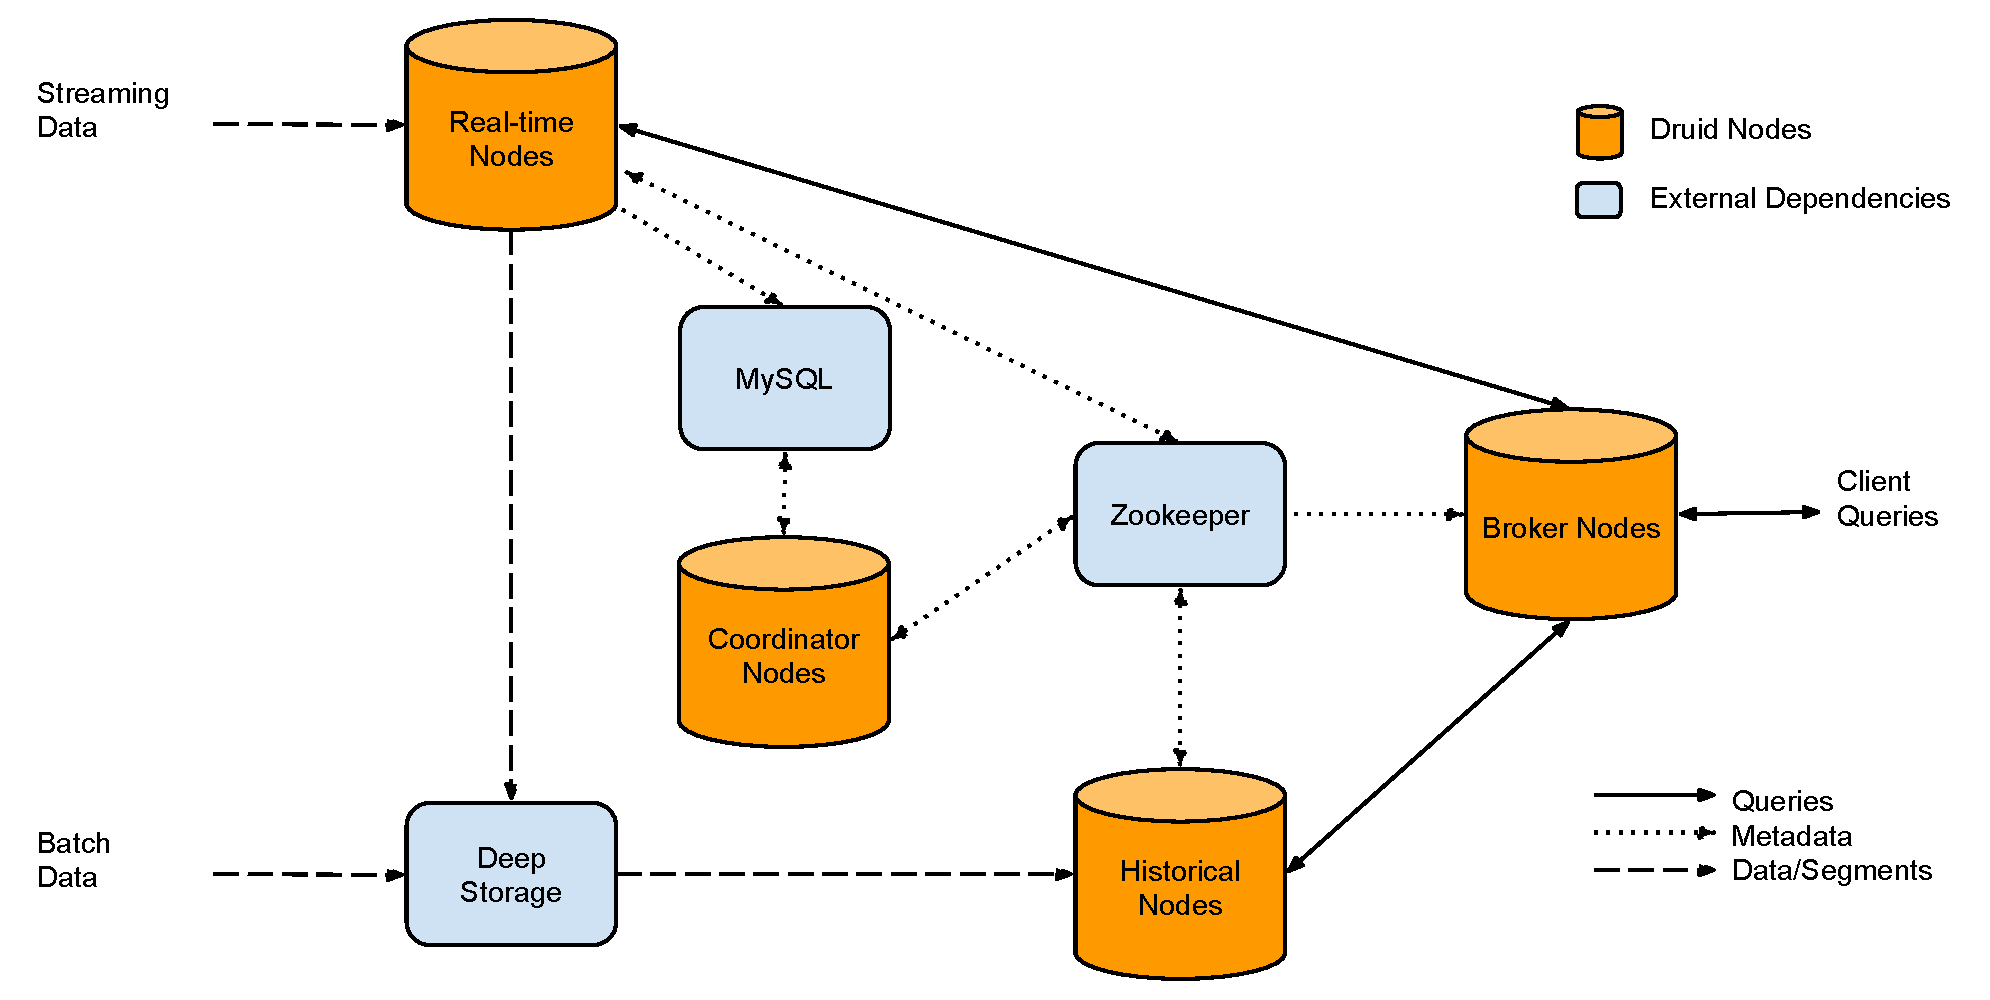
\includegraphics[width = 4.5in]{cluster}
\caption{An overview of a Druid cluster and the flow of data through the cluster.}
\label{fig:cluster}
\end{figure*}

\subsection{Real-time Nodes}
\label{sec:realtime}
Real-time nodes encapsulate the functionality to ingest and query event
streams. Events indexed via these nodes are immediately available for querying.
The nodes are only concerned with events for some small time range and
periodically hand off immutable batches of events they've collected over this
small time range to other nodes in the Druid cluster that are specialized in
dealing with batches of immutable events. Real-time nodes leverage Zookeeper
\cite{hunt2010zookeeper} for coordination with the rest of the Druid cluster.
The nodes announce their online state and the data they are serving in
Zookeeper. 

Real-time nodes maintain an in-memory index buffer for all incoming events.
These indexes are incrementally populated as new events are ingested and the
indexes are also directly queryable.  Druid virtually behaves as a row store
for queries on events that exist in this JVM heap-based buffer. To avoid heap overflow
problems, real-time nodes persist their in-memory indexes to disk either
periodically or after some maximum row limit is reached. This persist process
converts data stored in the in-memory buffer to a column oriented storage
format described in \ref{sec:storage-format}. Each persisted index is immutable and
real-time nodes load persisted indexes into off-heap memory such that they can
still be queried. Figure~\ref{fig:realtime_flow} illustrates the process.

\begin{figure} 
\centering 
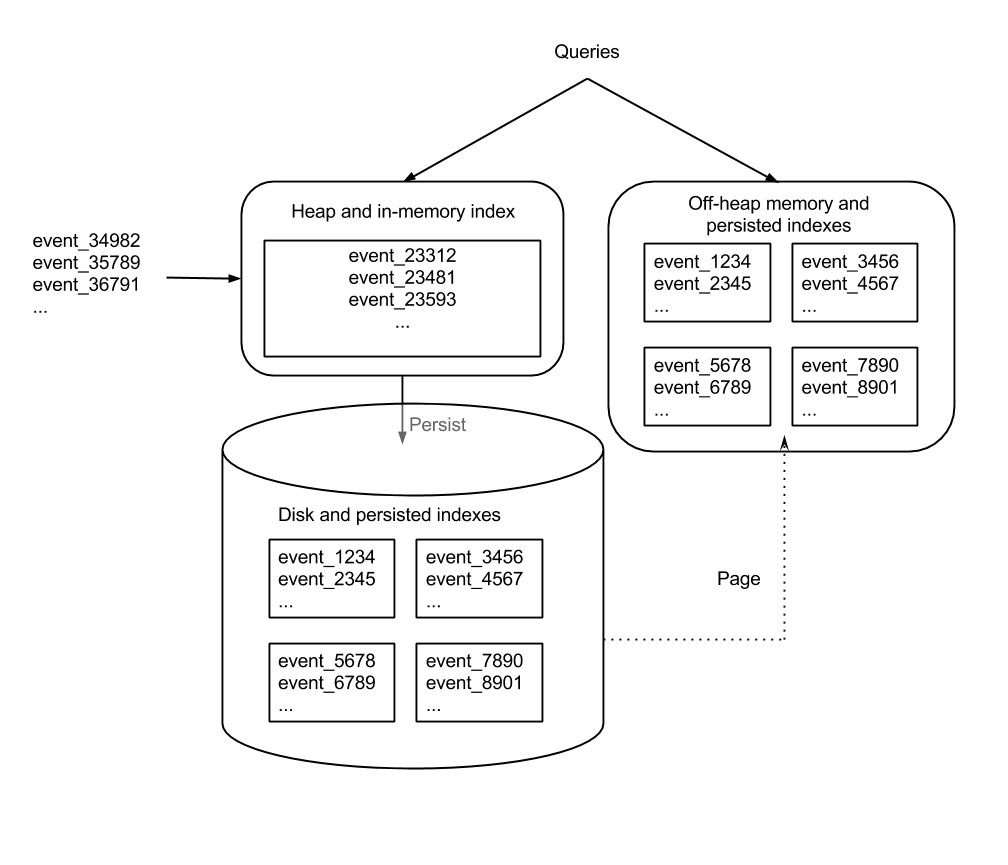
\includegraphics[width = 2.8in]{realtime_flow}
\caption{Real-time nodes first buffer events in memory. On a periodic basis,
the in-memory index is persisted to disk. On another periodic basis, all
persisted indexes are merged together and handed off. Queries for data will hit the
in-memory index and the persisted indexes.}
\label{fig:realtime_flow}
\end{figure}

On a periodic basis, each real-time node will schedule a background task that
searches for all locally persisted indexes. The task merges these indexes
together and builds an immutable block of data that contains all the events
that have ingested by a real-time node for some span of time. We refer to this
block of data as a "segment". During the handoff stage, a real-time node
uploads this segment to a permanent backup storage, typically a distributed
file system such as S3 \cite{decandia2007dynamo} or HDFS
\cite{shvachko2010hadoop}, which Druid refers to as "deep storage". The ingest,
persist, merge, and handoff steps are fluid; there is no data loss during any
of the processes.

To better understand the flow of data through a real-time node, consider the
following example. First, we start a real-time node at 13:37. The node will
only accept events for the current hour or the next hour. When the node begins
ingesting events, it will announce that it is serving a segment of data for a
time window from 13:00 to 14:00.  Every 10 minutes (the persist period is
configurable), the node will flush and persist its in-memory buffer to disk.
Near the end of the hour, the node will likely see events with timestamps from
14:00 to 15:00. When this occurs, the node prepares to serve data for the next
hour and creates a new in-memory index. The node then announces that it is also
serving a segment for data from 14:00 to 15:00.  The node does not immediately
merge the indexes it persisted from 13:00 to 14:00, instead it waits for a
configurable window period for straggling events from 13:00 to 14:00 to come
in. Having a window period minimizes the risk of data loss from delays in event
delivery. At the end of the window period, the real-time node merges all
persisted indexes from 13:00 to 14:00 into a single immutable segment and hands
the segment off.  Once this segment is loaded and queryable somewhere else in
the Druid cluster, the real-time node flushes all information about the data it
collected for 13:00 to 14:00 and unannounces it is serving this data. This
process is shown in Figure~\ref{fig:realtime_timeline}. 

\begin{figure*}
\centering
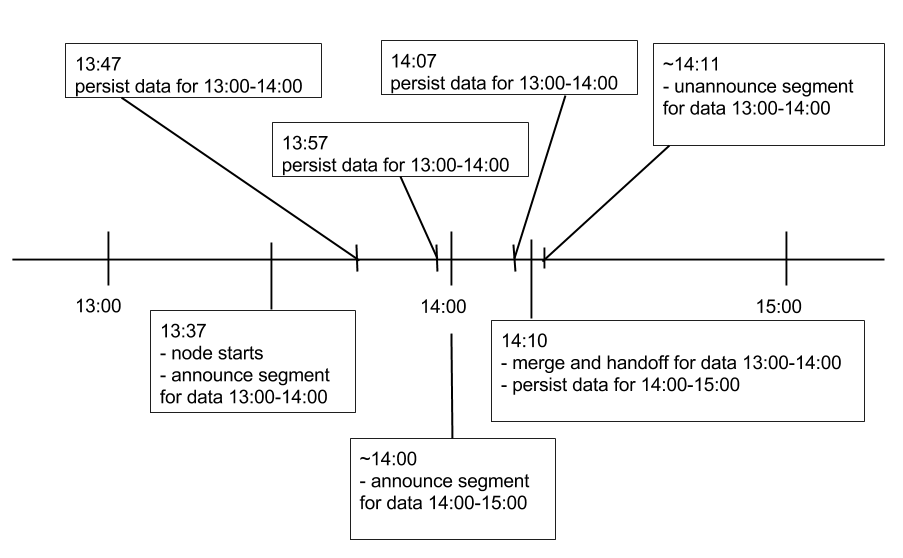
\includegraphics[width = 4.5in]{realtime_timeline}
\caption{The node starts, ingests data, persists, and periodically hands data
off. This process repeats indefinitely. The time intervals between different
real-time node operations are configurable.}
\label{fig:realtime_timeline}
\end{figure*}

\subsubsection{Availability and Scalability}
Real-time nodes are a consumer of data and require a corresponding producer to
provide the data stream.  Commonly, for data durability purposes, a message
bus such as Kafka \cite{kreps2011kafka} sits between the producer and the
real-time node as shown in Figure~\ref{fig:realtime_pipeline}. Real-time nodes
ingest data by reading events from the message bus. The time from event
creation to event consumption is ordinarily on the order of hundreds of
milliseconds.

\begin{figure}
\centering
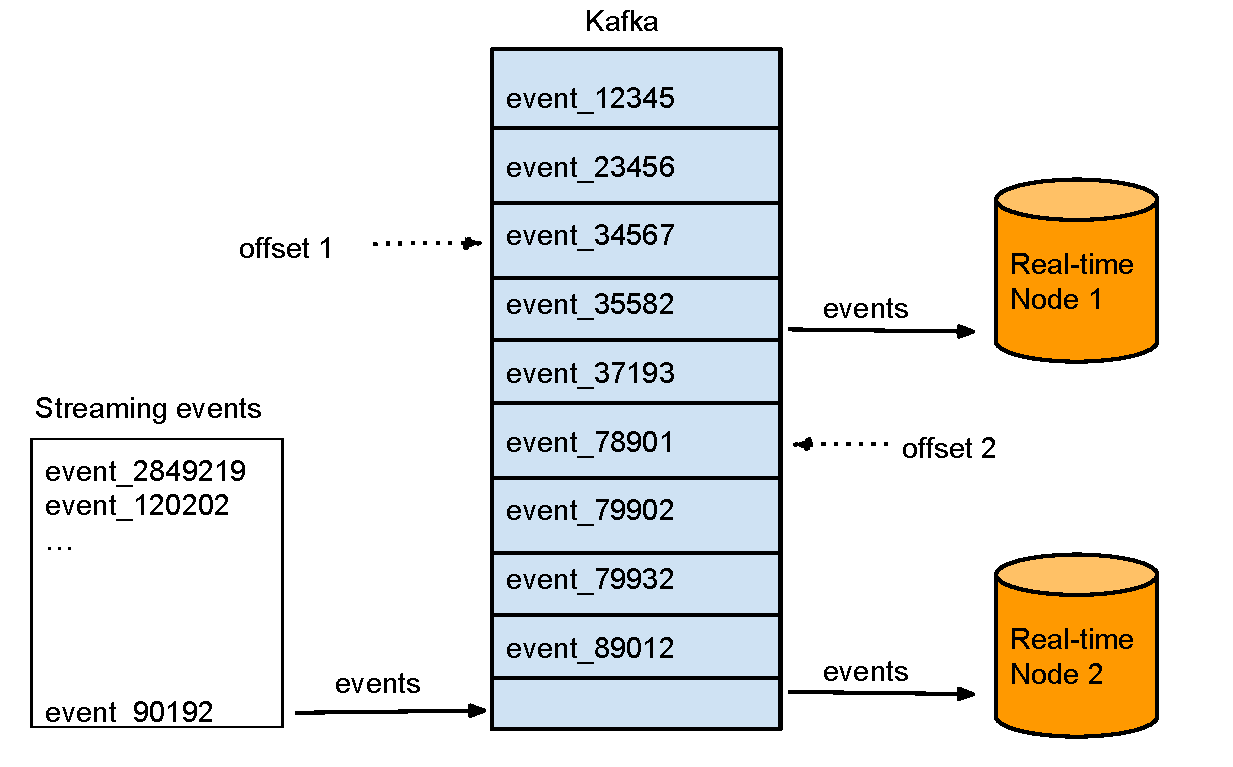
\includegraphics[width = 2.8in]{realtime_pipeline}
\caption{Multiple real-time nodes can read from the same message bus. Each node maintains its own offset.}
\label{fig:realtime_pipeline}
\end{figure}

The purpose of the message bus in Figure~\ref{fig:realtime_pipeline} is
two-fold.  First, the message bus acts as a buffer for incoming events. A
message bus such as Kafka maintains offsets indicating the position in an event
stream that a consumer (a real-time node) has read up to and consumers can
programmatically update these offsets. Typically, real-time nodes update this
offset each time they persist their in-memory buffers to disk. In a fail and
recover scenario, if a node has not lost disk, it can reload all persisted
indexes from disk and continue reading events from the last offset it
committed. Ingesting events from a recently committed offset greatly reduces a
node's recovery time. In practice, we see real-time nodes recover from such
failure scenarios in an order of seconds.

The second purpose of the message bus is to act as a single endpoint from which
multiple real-time nodes can read events. Multiple real-time nodes can ingest
the same set of events from the bus, thus creating a replication of events. In
a scenario where a node completely fails and does not recover, replicated
streams ensure that no data is lost. A single ingestion endpoint also allows
for data streams for be partitioned such that multiple real-time nodes each
ingest a portion of a stream. This allows additional real-time nodes to be
seamlessly added. In practice, this model has allowed one of the largest
production Druid clusters to be able to consume raw data at approximately 500
MB/s (150,000 events/s or 2 TB/hour).

\subsection{Historical Nodes}
Historical nodes encapsulate the functionality to load and serve the immutable
blocks of data (segments) created by real-time nodes. In many real-world
workflows, most of the data loaded in a Druid cluster is immutable and hence,
historical nodes are typically the main workers of a Druid cluster.  Historical
nodes follow a shared-nothing architecture and there is no single point of
contention among the nodes. The nodes have no knowledge of one another and are
operationally simple; they only know how to load, drop, and serve immutable
segments. 

Similar to real-time nodes, historical nodes announce their online state and
the data they are serving in Zookeeper. Instructions to load and drop segments
are sent over Zookeeper and contain information about where the segment is
located in deep storage and how to decompress and process the segment.  Before
a historical node downloads a particular segment from deep storage, it first
checks a local cache that maintains information about what segments already
exist on the node.  If information about a segment is not present in the cache,
the historical node will proceed to download the segment from deep storage.
This process is shown in Figure~\ref{fig:historical_download}. Once processing
is complete, the segment is announced in Zookeeper.  At this point, the segment
is queryable. The local cache also allows for historical nodes to be quickly
updated and restarted. On startup, the node examines its cache and immediately
serves whatever data it finds.

\begin{figure}
\centering
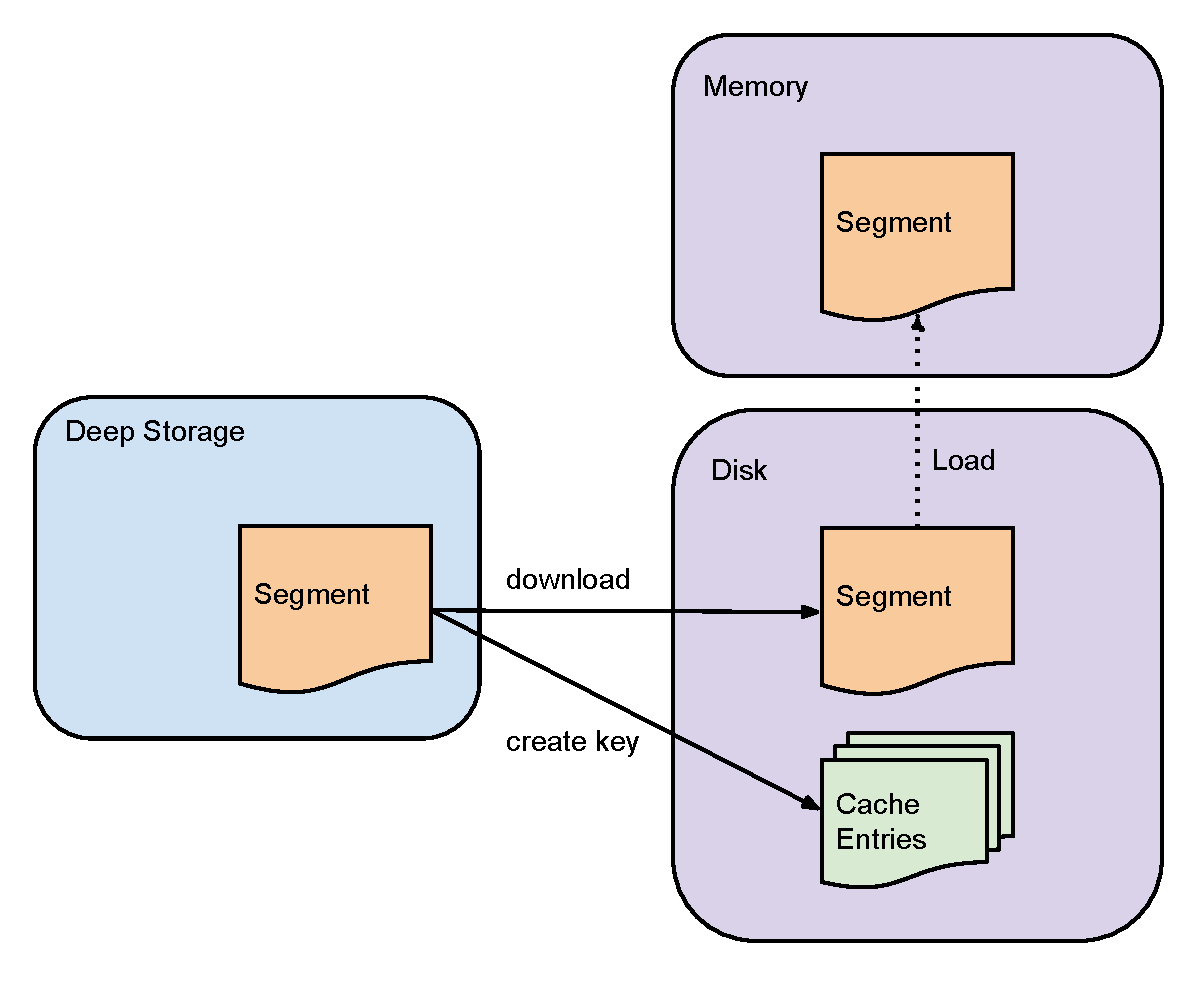
\includegraphics[width = 2.6in]{historical_download}
\caption{Historical nodes download immutable segments from deep storage. Segments must be loaded in memory before they can be queried.}
\label{fig:historical_download}
\end{figure}

Historical nodes can support read consistency because they only deal with
immutable data. Immutable data blocks also enable a simple parallelization
model: historical nodes can concurrently scan and aggregate immutable blocks
without blocking.
 
\subsubsection{Tiers}
\label{sec:tiers}
Historical nodes can be grouped in different tiers, where all nodes in a
given tier are identically configured. Different performance and
fault-tolerance parameters can be set for each tier. The purpose of
tiered nodes is to enable higher or lower priority segments to be
distributed according to their importance. For example, it is possible
to spin up a “hot” tier of historical nodes that have a high number of
cores and large memory capacity. The “hot” cluster can be configured to
download more frequently accessed data. A parallel “cold” cluster
can also be created with much less powerful backing hardware. The
“cold” cluster would only contain less frequently accessed segments.

\subsubsection{Availability}
Historical nodes depend on Zookeeper for segment load and unload instructions.
If Zookeeper becomes unavailable, historical nodes are no longer able to serve
new data and drop outdated data, however, because the queries are served over
HTTP, historical nodes are still be able to respond to query requests for
the data they are currently serving. This means that Zookeeper outages do not
impact current data availability on historical nodes. 

\subsection{Broker Nodes}
Broker nodes act as query routers to historical and real-time nodes. Broker
nodes understand the metadata published in Zookeeper about what segments are
queryable and where those segments are located. Broker nodes route incoming queries
such that the queries hit the right historical or real-time nodes. Broker nodes
also merge partial results from historical and real-time nodes before returning
a final consolidated result to the caller.  

\subsubsection{Caching}
\label{sec:caching}
Broker nodes contain a cache with a LRU \cite{o1993lru, kim2001lrfu}
invalidation strategy. The cache can use local heap memory or an external
distributed key/value store such as memcached
\cite{fitzpatrick2004distributed}. Each time a broker node receives a query, it
first maps the query to a set of segments. Results for certain segments may
already exist in the cache and there is no need to recompute them. For any
results that do not exist in the cache, the broker node will forward the query
to the correct historical and real-time nodes.  Once historical nodes return
their results, the broker will cache these results on a per segment basis for
future use. This process is illustrated in Figure~\ref{fig:caching}. Real-time
data is never cached and hence requests for real-time data will always be
forwarded to real-time nodes.  Real-time data is perpetually changing and
caching the results would be unreliable.

\begin{figure*}
\centering
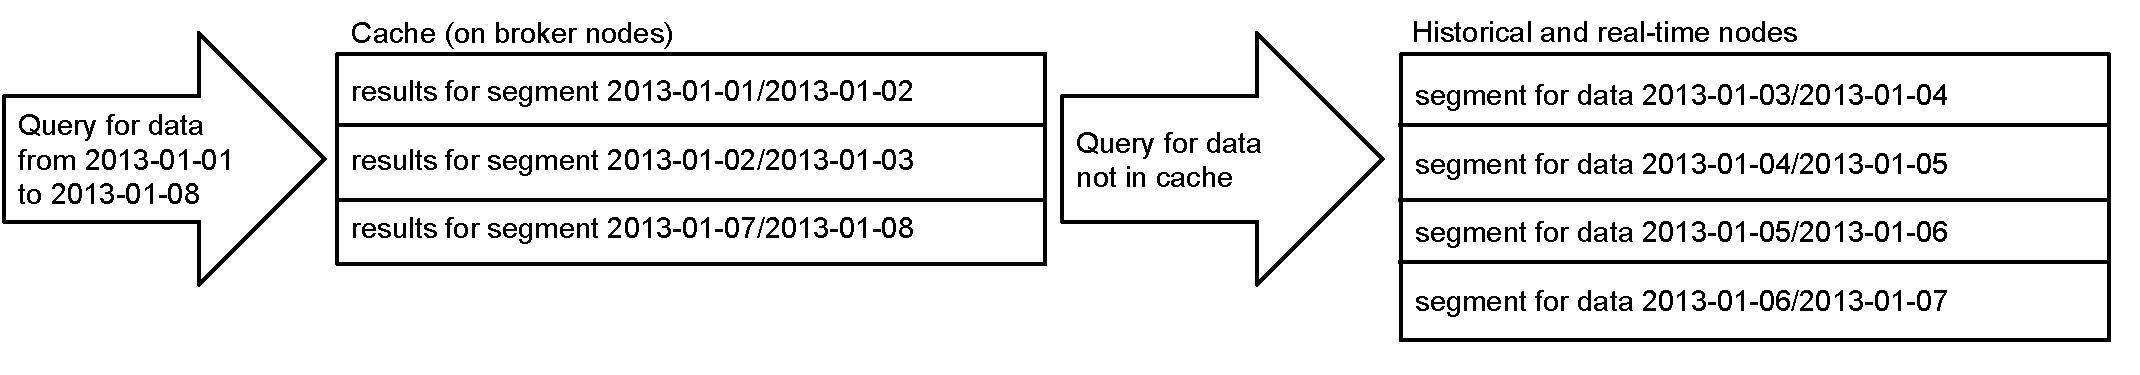
\includegraphics[width = 4.5in]{caching}
\caption{Broker nodes cache per segment results. Every Druid query is mapped to
a set of segments. Queries often combine cached segment results with those that
need to be computed on historical and real-time nodes.}
\label{fig:caching}
\end{figure*}

The cache also acts as an additional level of data durability. In the event
that all historical nodes fail, it is still possible to query results if those
results already exist in the cache.

\subsubsection{Availability}
In the event of a total Zookeeper outage, data is still queryable.  If broker
nodes are unable to communicate to Zookeeper, they use their last known view of
the cluster and continue to forward queries to real-time and historical nodes.
Broker nodes make the assumption that the structure of the cluster is the same
as it was before the outage. In practice, this availability model has allowed
our Druid cluster to continue serving queries for a significant period of time while we
diagnosed Zookeeper outages. 

\subsection{Coordinator Nodes}
Druid coordinator nodes are primarily in charge of data management and
distribution on historical nodes. The coordinator nodes tell historical nodes
to load new data, drop outdated data, replicate data, and move data to load
balance. Druid uses a multi-version concurrency control swapping protocol for
managing immutable segments in order to maintain stable views.  If any
immutable segment contains data that is wholly obseleted by newer segments, the
outdated segment is dropped from the cluster. Coordinator nodes undergo a
leader-election process that determines a single node that runs the coordinator
functionality. The remaining coordinator nodes act as redundant backups.

A coordinator node runs periodically to determine the current state of the
cluster. It makes decisions by comparing the expected state of the cluster with
the actual state of the cluster at the time of the run. As with all Druid
nodes, coordinator nodes maintain a Zookeeper connection for current cluster
information. Coordinator nodes also maintain a connection to a MySQL
database that contains additional operational parameters and configurations.
One of the key pieces of information located in the MySQL database is a table
that contains a list of all segments that should be served by historical nodes.
This table can be updated by any service that creates segments, for example,
real-time nodes. The MySQL database also contains a rule table that governs how
segments are created, destroyed, and replicated in the cluster.

\subsubsection{Rules}
Rules govern how historical segments are loaded and dropped from the cluster.
Rules indicate how segments should be assigned to different historical node
tiers and how many replicates of a segment should exist in each tier. Rules may
also indicate when segments should be dropped entirely from the cluster. Rules
are usually set for a period of time.  For example, a user may use rules to
load the most recent one month's worth of segments into a "hot" cluster, the
most recent one year's worth of segments into a "cold" cluster, and drop any
segments that are older.

The coordinator nodes load a set of rules from a rule table in the MySQL
database. Rules may be specific to a certain data source and/or a default set
of rules may be configured. The coordinator node will cycle through all available
segments and match each segment with the first rule that applies to it.

\subsubsection{Load Balancing}
In a typical production environment, queries often hit dozens or even hundreds
of segments. Since each historical node has limited resources, segments must be
distributed among the cluster to ensure that the cluster load is not too
imbalanced. Determining optimal load distribution requires some knowledge about
query patterns and speeds. Typically, queries cover recent segments spanning
contiguous time intervals for a single data source.  On average, queries that
access smaller segments are faster.

These query patterns suggest replicating recent historical segments at a higher
rate, spreading out large segments that are close in time to different
historical nodes, and co-locating segments from different data sources.  To
optimally distribute and balance segments among the cluster, we developed a
cost-based optimization procedure that takes into account the segment data
source, recency, and size. The exact details of the algorithm are beyond the
scope of this paper and may be discussed in future literature.

\subsubsection{Replication}
Coordinator nodes may tell different historical nodes to load copies of the
same segment. The number of replicates in each tier of the historical compute
cluster is fully configurable. Setups that require high levels of fault
tolerance can be configured to have a high number of replicas. Replicated
segments are treated the same as the originals and follow the same load
distribution algorithm. By replicating segments, single historical node
failures are transparent in the Druid cluster. We use this property for
software upgrades. We can seamlessly take a historical node offline, update it,
bring it back up, and repeat the process for every historical node in a
cluster. Over the last two years, we have never taken downtime in our Druid
cluster for software upgrades.

\subsubsection{Availability}
Druid coordinator nodes have two external dependencies: Zookeeper and MySQL.
Coordinator nodes rely on Zookeeper to determine what historical nodes already
exist in the cluster. If Zookeeper becomes unavailable, the coordinator will no
longer be able to send instructions to assign, balance, and drop segments.
However, these operations do not affect data availability at all.

The design principle for responding to MySQL and Zookeeper failures is the
same: if an external dependency responsible for coordination fails, the cluster
maintains the status quo. Druid uses MySQL to store operational management
information and segment metadata information about what segments should exist
in the cluster.  If MySQL goes down, this information becomes unavailable to
coordinator nodes. However, this does not mean data itself is unavailable. If
coordinator nodes cannot communicate to MySQL, they will cease to assign new
segments and drop outdated ones. Broker, historical and real-time nodes are still
queryable during MySQL outages.

\section{Storage Format}
\label{sec:storage-format}
Data tables in Druid (called \emph{data sources}) are collections of
timestamped events and partitioned into a set of segments, where each segment
is typically 5--10 million rows. Formally, we define a segment as a collection
of rows of data that span some period in time. Segments represent the
fundamental storage unit in Druid and replication and distribution are done at
a segment level.
 
Druid always requires a timestamp column as a method of simplifying data
distribution policies, data retention policies, and first-level query pruning.
Druid partitions its data sources into well-defined time intervals, typically
an hour or a day, and may further partition on values from other columns to
achieve the desired segment size.  For example, partitioning the data in
Table~\ref{tab:sample_data} by hour results in two segments for 2011-01-01, and
partitioning the data by day results in a single segment.  The time granularity
to partition segments is a function of data volume and time range. A data set
with timestamps spread over a year is better partitioned by day, and a data set
with timestamps spread over a day is better partitioned by hour.

Segments are uniquely identified by a data source identifer, the time interval
of the data, and a version string that increases whenever a new segment is
created.  The version string indicates the freshness of segment data; segments
with later versions have newer views of data (over some time range) than
segments with older versions.  This segment metadata is used by the system for
concurrency control; read operations always access data in a particular time
range from the segments with the latest version identifiers for that time
range.

Druid segments are stored in a column orientation. Given that Druid is best
used for aggregating event streams (all data going into Druid must have a
timestamp), the advantages storing aggregate information as columns rather than
rows are well documented \cite{abadi2008column}. Column storage allows for more
efficient CPU usage as only what is needed is actually loaded and scanned. In a
row oriented data store, all columns associated with a row must be scanned as
part of an aggregation. The additional scan time can introduce signficant performance
degradations \cite{abadi2008column}.

Druid has multiple column types to represent various data formats. Depending on
the column type, different compression methods are used to reduce the cost of
storing a column in memory and on disk. In the example given in
Table~\ref{tab:sample_data}, the page, user, gender, and city columns only
contain strings. Storing strings directly is unnecessarily costly and string
columns can be dictionary encoded instead. Dictionary encoding is a common
method to compress data and has been used in other data stores such as
PowerDrill \cite{hall2012processing}. In the example in
Table~\ref{tab:sample_data}, we can map each publisher to an unique integer
identifier.
\begin{verbatim}
Justin Bieber   -> 0
Ke$ha -> 1
\end{verbatim}
This mapping allows us to represent the page column as an integer
array where the array indices correspond to the rows of the original
data set. For the page column, we can represent the unique
pages as follows:
\begin{verbatim}
[0, 0, 1, 1]
\end{verbatim}

The resulting integer array lends itself very well to
compression methods. Generic compression algorithms on top of encodings are
extremely common in column-stores. Druid uses the LZF \cite{liblzf2013} compression
algorithm.

Similar compression methods can be applied to numeric
columns. For example, the characters added and characters removed columns in
Table~\ref{tab:sample_data} can also be expressed as individual
arrays.
\begin{verbatim}
Characters Added  -> [1800, 2912, 1953, 3194]
Characters Removed -> [25, 42, 17, 170]
\end{verbatim}
In this case, we compress the raw values as opposed to their dictionary
representations.

\subsection{Indices for Filtering Data}
In many real world OLAP workflows, queries are issued for the aggregated
results of some set of metrics where some set of dimension specifications are
met. An example query may be asked is: "How many Wikipedia edits were done by users in
San Francisco who are also male?". This query is filtering the Wikipedia data
set in Table~\ref{tab:sample_data} based on a Boolean expression of dimension
values. In many real world data sets, dimension columns contain strings and
metric columns contain numeric values. Druid creates additional lookup
indices for string columns such that only those rows that pertain to a
particular query filter are ever scanned.

Let us consider the page column in
Table~\ref{tab:sample_data}. For each unique page in
Table~\ref{tab:sample_data}, we can form some representation
indicating in which table rows a particular page is seen. We can
store this information in a binary array where the array indices
represent our rows. If a particular page is seen in a certain
row, that array index is marked as \texttt{1}. For example:
\begin{verbatim}
Justin Bieber   -> rows [0, 1] -> [1][1][0][0]
Ke$ha -> rows [2, 3] -> [0][0][1][1]
\end{verbatim}

\texttt{Justin Bieber} is seen in rows \texttt{0} and \texttt{1}. This mapping of column values
to row indices forms an inverted index \cite{tomasic1993performance}. To know which
rows contain {\ttfamily Justin Bieber} or {\ttfamily Ke\$ha}, we can \texttt{OR} together
the two arrays.
\begin{verbatim}
[0][1][0][1] OR [1][0][1][0] = [1][1][1][1]
\end{verbatim}

\begin{figure}
\centering
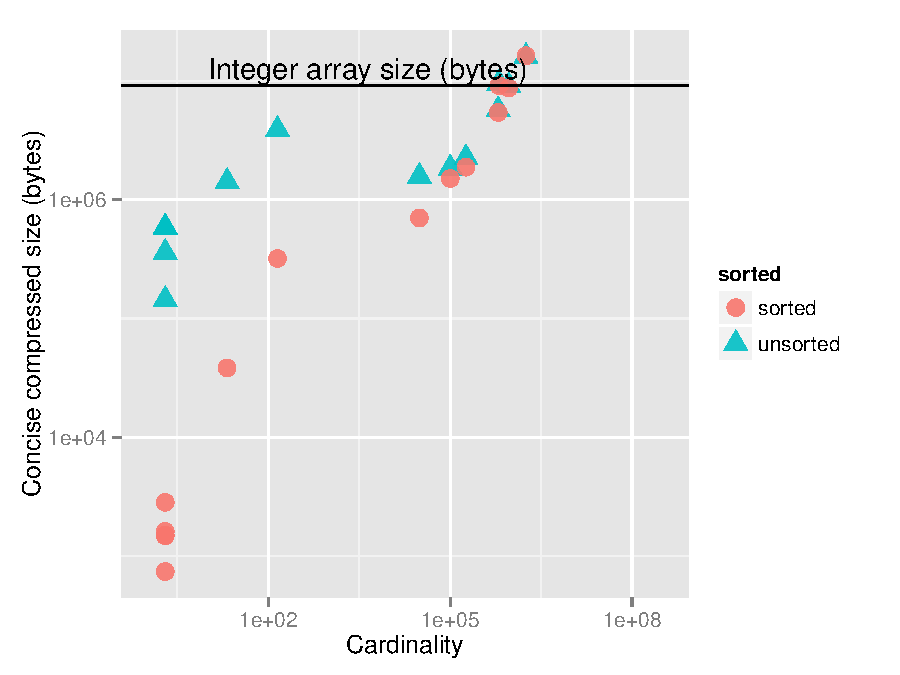
\includegraphics[width = 3in]{concise_plot}
\caption{Integer array size versus Concise set size.}
\label{fig:concise_plot}
\end{figure}

This approach of performing Boolean operations on large bitmap sets is commonly
used in search engines. Bitmap compression algorithms are a well-defined area
of research and often utilize run-length encoding. Popular algorithms include
Byte-aligned Bitmap Code \cite{antoshenkov1995byte}, Word-Aligned Hybrid (WAH)
code \cite{wu2006optimizing}, and Partitioned Word-Aligned Hybrid (PWAH)
compression \cite{van2011memory}. Druid opted to use the Concise algorithm
\cite{colantonio2010concise} as it can outperform WAH by reducing the size of
the compressed bitmaps by up to 50\%.  Figure~\ref{fig:concise_plot}
illustrates the number of bytes using Concise compression versus using an
integer array. The results were generated on a cc2.8xlarge system with a single
thread, 2G heap, 512m young gen, and a forced GC between each run. The data set
is a single day’s worth of data collected from the Twitter garden hose
\cite{twitter2013} data stream. The data set contains 2,272,295 rows and 12
dimensions of varying cardinality. As an additional comparison, we also
resorted the data set rows to maximize compression.

In the unsorted case, the total Concise size was 53,451,144 bytes and the total
integer array size was 127,248,520 bytes. Overall, Concise compressed sets are
about 42\% smaller than integer arrays.  In the sorted case, the total Concise
compressed size was 43,832,884 bytes and the total integer array size was
127,248,520 bytes.  What is interesting to note is that after sorting, global
compression only increased minimally. The total Concise set size to total
integer array size is 34\%. It is also interesting to note that as the
cardinality of a dimension approaches the total number of rows in a data set,
integer arrays require less space than Concise sets and become a better
alternative.

\subsection{Storage Engine}
Druid’s persistence components allows for different storage engines to be
plugged in, similar to Dynamo \cite{decandia2007dynamo}. These storage engines
may store data in an entirely in-memory structure such as the JVM heap or in
memory-mapped structures. The ability to swap storage engines allows for Druid
to be configured depending on a particular application’s specifications. An
in-memory storage engine may be operationally more expensive than a
memory-mapped storage engine but could be a better alternative if performance
is critical. By default, a memory-mapped storage engine is used.

When using a memory-mapped storage engine, Druid relies on the operating system
to page segments in and out of memory.  Given that segments can only be scanned
if they are loaded in memory, a memory-mapped storage engine allows recent
segments to retain in memory whereas segments that are never queried are paged
out. The main drawback with using the memory-mapped storage engine is when a
query requires more segments to be paged into memory than a given node has
capacity for. In this case, query performance will suffer from the cost of
paging segments in and out of memory.

\section{Query API}
\label{sec:query-api}
Druid has its own query language and accepts queries as POST requests. Broker,
historical, and real-time nodes all share the same query API.

The body of the POST request is a JSON object containing key-value pairs
specifying various query parameters. A typical query will contain the data
source name, the granularity of the result data, time range of interest, the
type of request, and the metrics to aggregate over. The result will also be a
JSON object containing the aggregated metrics over the time period.

Most query types will also support a filter set. A filter set is a Boolean
expression of dimension name and value pairs. Any number and combination of
dimensions and values may be specified.  When a filter set is provided, only
the subset of the data that pertains to the filter set will be scanned.  The
ability to handle complex nested filter sets is what enables Druid to drill
into data at any depth.

The exact query syntax depends on the query type and the information requested.
A sample count query over a week of data is shown below:
\begin{verbatim}
{
  "queryType"     : "timeseries",
  "dataSource"    : "wikipedia",
  "intervals"     : "2013-01-01/2013-01-08",
  "filter"        : {
    "type"        : "selector",
    "dimension"   : "page",
    "value"       : "Ke$ha"
  },
  "granularity"   : "day",
  "aggregations"  : [ {
      "type"      : "count",
      "name"      : "rows"
   } ]
}
\end{verbatim}

The query shown above will return a count of the number of rows in the Wikipedia datasource
from 2013-01-01 to 2013-01-08, filtered for only those rows where the value of the "page" dimension is 
equal to "Ke\$ha". The results will be bucketed by day and will be a JSON array of the following form:
\begin{verbatim}
[ {
    "timestamp": "2012-01-01T00:00:00.000Z",
    "result": {
      "rows": 393298
    }
  },
  {
    "timestamp": "2012-01-02T00:00:00.000Z",
    "result": {
      "rows": 382932
    }
  },
  ...
  {
    "timestamp": "2012-01-07T00:00:00.000Z",
    "result": {
      "rows": 1337
    }
} ]
\end{verbatim}

Druid supports many types of aggregations including double sums, long sums,
minimums, maximums, and several others. Druid also supports complex aggregations
such as cardinality estimation and approximate quantile estimation.  The
results of aggregations can be combined in mathematical expressions to form
other aggregations. The query API is highly customizable and can be extended to
filter and group results based on almost any arbitrary condition.  It is beyond
the scope of this paper to fully describe the query API but more information
can be found
online\footnote{\href{http://druid.io/docs/latest/Querying.html}{http://druid.io/docs/latest/Querying.html}}.
We are also in the process of extending the Druid API to understand SQL.

\section{Performance Benchmarks}
\label{sec:benchmarks}
To illustrate Druid's performance, we conducted a series of experiments that
focused on measuring Druid's query and data ingestion capabilities.

\subsection{Query Performance}
To benchmark Druid query performance, we created a large test cluster with 6TB
of uncompressed data, representing tens of billions of fact rows. The data set
contained more than a dozen dimensions, with cardinalities ranging from the
double digits to tens of millions. We computed four metrics for each row
(counts, sums, and averages). The data was sharded first on timestamp and then
on dimension values, creating thousands of shards roughly 8 million fact rows
apiece.

The cluster used in the benchmark consisted of 100 historical nodes, each with
16 cores, 60GB of RAM, 10 GigE Ethernet, and 1TB of disk space. Collectively,
the cluster comprised of 1600 cores, 6TB or RAM, sufficiently fast Ethernet and
more than enough disk space.

SQL statements are included in Table~\ref{tab:sql_queries}. These queries are
meant to represent some common queries that are made against Druid for typical data
analysis workflows. Although Druid has its own query language, we choose to
translate the queries into SQL to better describe what the queries are doing.
Please note:
\begin{itemize}
\item The timestamp range of the queries encompassed all data.
\item Each machine was a 16-core machine with 60GB RAM and 1TB of local
  disk. The machine was configured to only use 15 threads for
  processing queries.
\item A memory-mapped storage engine was used (the machine was configured to memory map the data
  instead of loading it into the Java heap.)
\end{itemize}

\begin{table*}
  \centering
  \caption{Druid Queries}
  \label{tab:sql_queries}
  \begin{tabular}{| l | p{15cm} |}
    \hline
    \textbf{Query \#} & \textbf{Query} \\ \hline
    1 & \texttt{SELECT count(*) FROM \_table\_ WHERE timestamp $\geq$ ? AND timestamp < ?} \\ \hline
    2 & \texttt{SELECT count(*), sum(metric1) FROM \_table\_ WHERE timestamp $\geq$ ? AND timestamp < ?} \\ \hline
    3 & \texttt{SELECT count(*), sum(metric1), sum(metric2), sum(metric3), sum(metric4) FROM \_table\_ WHERE timestamp $\geq$ ? AND timestamp < ?} \\ \hline
    4 & \texttt{SELECT high\_card\_dimension, count(*) AS cnt FROM \_table\_ WHERE timestamp $\geq$ ? AND timestamp < ? GROUP BY high\_card\_dimension ORDER BY cnt limit 100} \\ \hline
    5 & \texttt{SELECT high\_card\_dimension, count(*) AS cnt, sum(metric1) FROM \_table\_ WHERE timestamp $\geq$ ? AND timestamp < ? GROUP BY high\_card\_dimension ORDER BY cnt limit 100} \\ \hline
    6 & \texttt{SELECT high\_card\_dimension, count(*) AS cnt, sum(metric1), sum(metric2), sum(metric3), sum(metric4) FROM \_table\_ WHERE timestamp $\geq$ ? AND timestamp < ? GROUP BY high\_card\_dimension ORDER BY cnt limit 100} \\ \hline
  \end{tabular}
\end{table*}

Figure~\ref{fig:cluster_scan_rate} shows the cluster scan rate and
Figure~\ref{fig:core_scan_rate} shows the core scan rate.  In
Figure~\ref{fig:cluster_scan_rate} we also include projected linear scaling
based on the results of the 25 core cluster.  In particular, we observe
diminishing marginal returns to performance in the size of the cluster.  Under
linear scaling, the first SQL count query (query 1) would have achieved a speed
of 37 billion rows per second on our 75 node cluster.  In fact, the speed was
26 billion rows per second.  However, queries 2-6 maintain a near-linear
speedup up to 50 nodes: the core scan rates in Figure~\ref{fig:core_scan_rate}
remain nearly constant.  The increase in speed of a parallel computing system
is often limited by the time needed for the sequential operations of the
system, in accordance with Amdahl's law \cite{amdahl1967validity}.

\begin{figure}
\centering
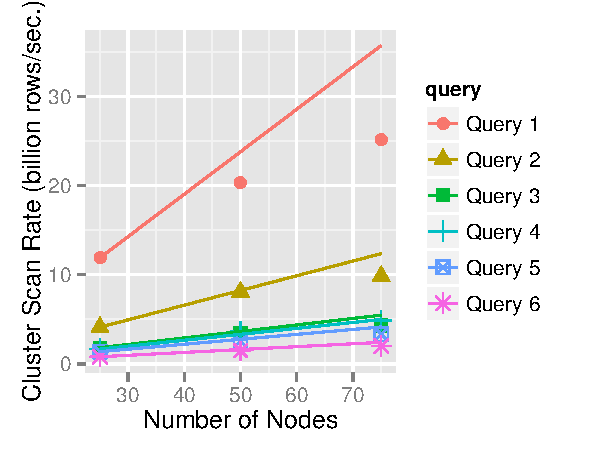
\includegraphics[width = 2.8in]{cluster_scan_rate}
\caption{Druid cluster scan rate with lines indicating linear scaling
  from 25 nodes.}
\label{fig:cluster_scan_rate}
\end{figure}

\begin{figure}
\centering
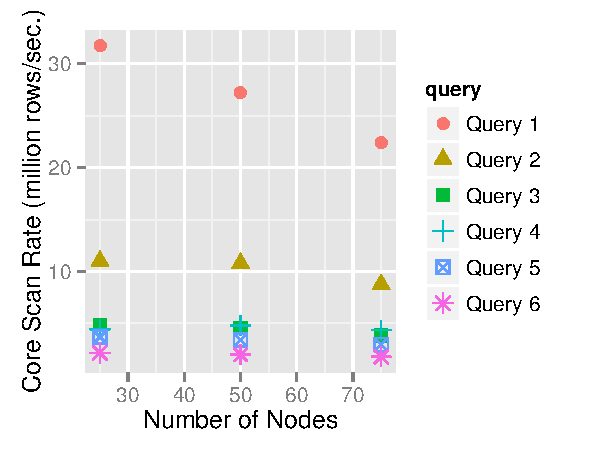
\includegraphics[width = 2.8in]{core_scan_rate}
\caption{Druid core scan rate.}
\label{fig:core_scan_rate}
\end{figure}

The first query listed in Table~\ref{tab:sql_queries} is a simple
count, achieving scan rates of 33M rows/second/core. We believe
the 75 node cluster was actually overprovisioned for the test
dataset, explaining the modest improvement over the 50 node cluster.
Druid's concurrency model is based on shards: one thread will scan one
shard. If the number of segments on a historical node modulo the number
of cores is small (e.g. 17 segments and 15 cores), then many of the
cores will be idle during the last round of the computation.

When we include more aggregations we see performance degrade.  This is
because of the column-oriented storage format Druid employs.  For the
\texttt{count(*)} queries, Druid only has to check the timestamp column to satisfy
the ``where'' clause.  As we add metrics, it has to also load those metric
values and scan over them, increasing the amount of memory scanned.

\subsection{Data Ingestion Performance}
To measure Druid's data latency latency, we spun up a single real-time node
with the following configurations:
\begin{itemize}
\item JVM arguments: -Xmx2g -Duser.timezone=UTC -Dfile.encoding=UTF-8 -XX:+HeapDumpOnOutOfMemoryError
\item CPU: 2.3 GHz Intel Core i7 
\end{itemize}

Druid's data ingestion latency is heavily dependent on the complexity of the
data set being ingested. The data complexity is determined by the number of
dimensions in each event, the number of metrics in each event, and the types of
aggregations we want to perform on those metrics. With the most basic data set
(one that only has a timestamp column), our setup can ingest data at a rate of
800k events/sec/node, which is really just a measurement of how fast we can
deserialize events. Real world data sets are never this simple. To simulate
real-world ingestion rates, we created a data set with 5 dimensions and a
single metric. 4 out of the 5 dimensions have a cardinality less than 100, and
we varied the cardinality of the final dimension. The results of varying the
cardinality of a dimension is shown in
Figure~\ref{fig:throughput_vs_cardinality}.

\begin{figure}
\centering
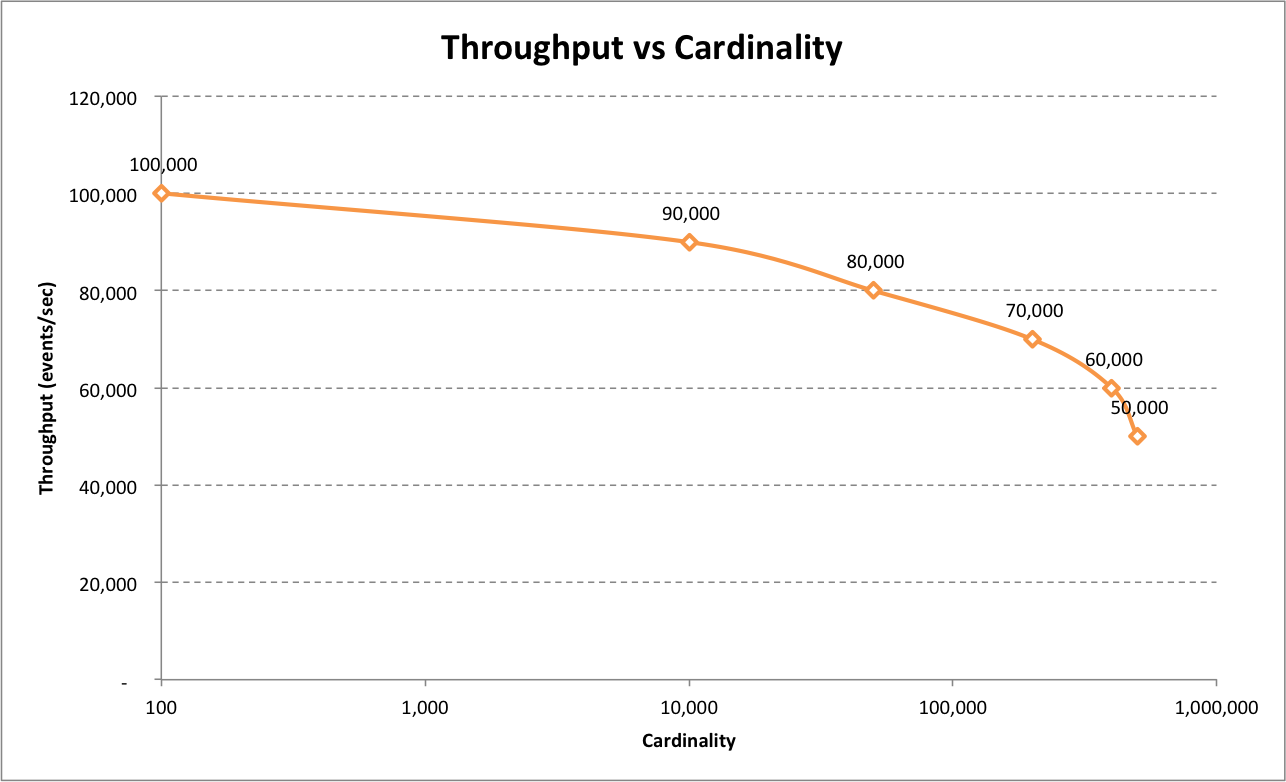
\includegraphics[width = 2.8in]{throughput_vs_cardinality}
\caption{When we vary the cardinality of a single dimension, we can see monotonically decreasing throughput.}
\label{fig:throughput_vs_cardinality}
\end{figure}

In Figure~\ref{fig:throughput_vs_num_dims}, we instead vary the number of
dimensions in our data set. Each dimension has a cardinality less than 100. We
can see a similar decline in ingestion throughput as the number of dimensions
increases.

\begin{figure}
\centering
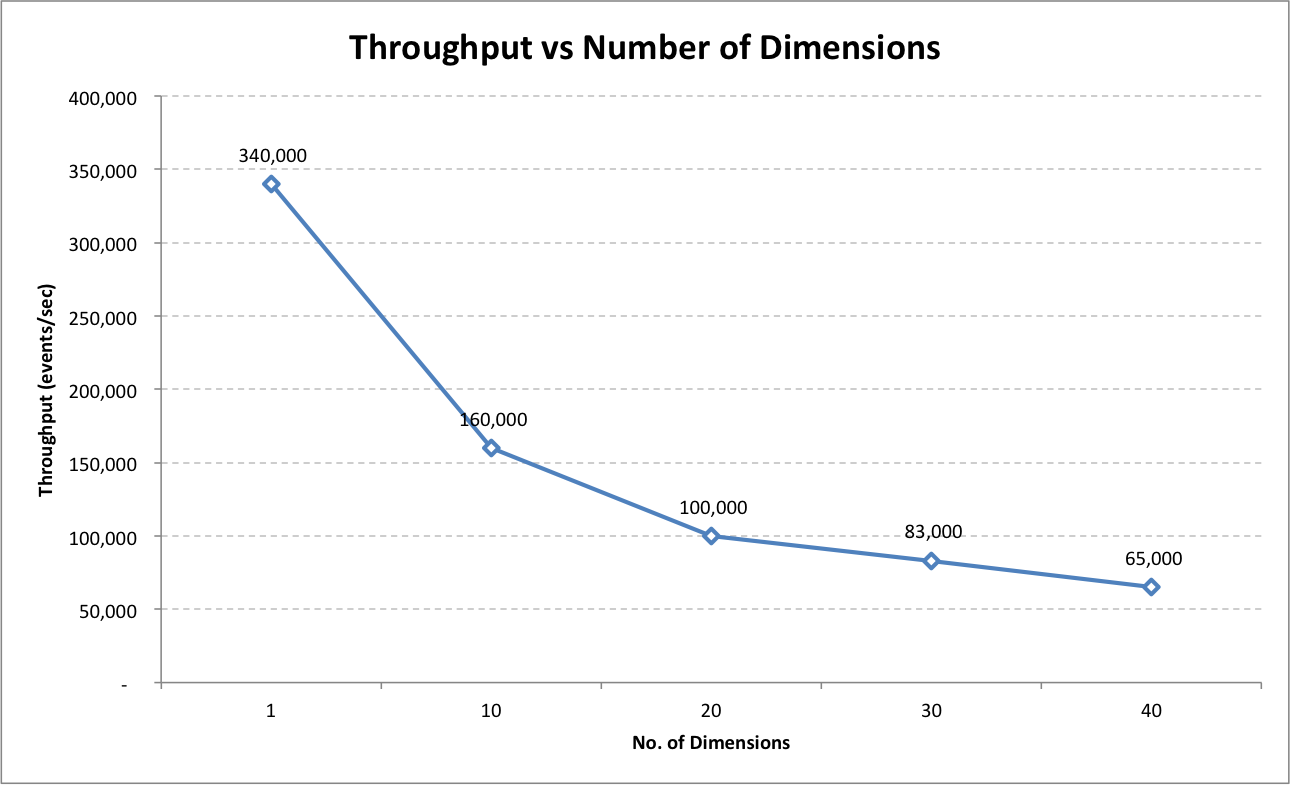
\includegraphics[width = 2.8in]{throughput_vs_num_dims}
\caption{Increasing the number of dimensions of our data set also leads to a decline in throughput.}
\label{fig:throughput_vs_num_dims}
\end{figure}

Finally, keeping our number of dimensions constant at 5, with four dimensions
having a cardinality in the 0-100 range and the final dimension having a
cardinality of 10,000, we can see a similar decline in throughput when we
increase the number of metrics/aggregators in the data set. We used random
types of metrics/aggregators in this experiment, and they vary from longs,
doubles, and other more complex types. The randomization introduces more noise
in the results, leading to a graph that is not strictly decreasing. These
results are shown in Figure~\ref{fig:throughput_vs_num_metrics}. For most real
world data sets, the number of metrics tends to be less than the number of
dimensions.  Hence, we can see that introducing a few new metrics does not
impact the ingestion latency as severely as in the other graphs.

\begin{figure}
\centering
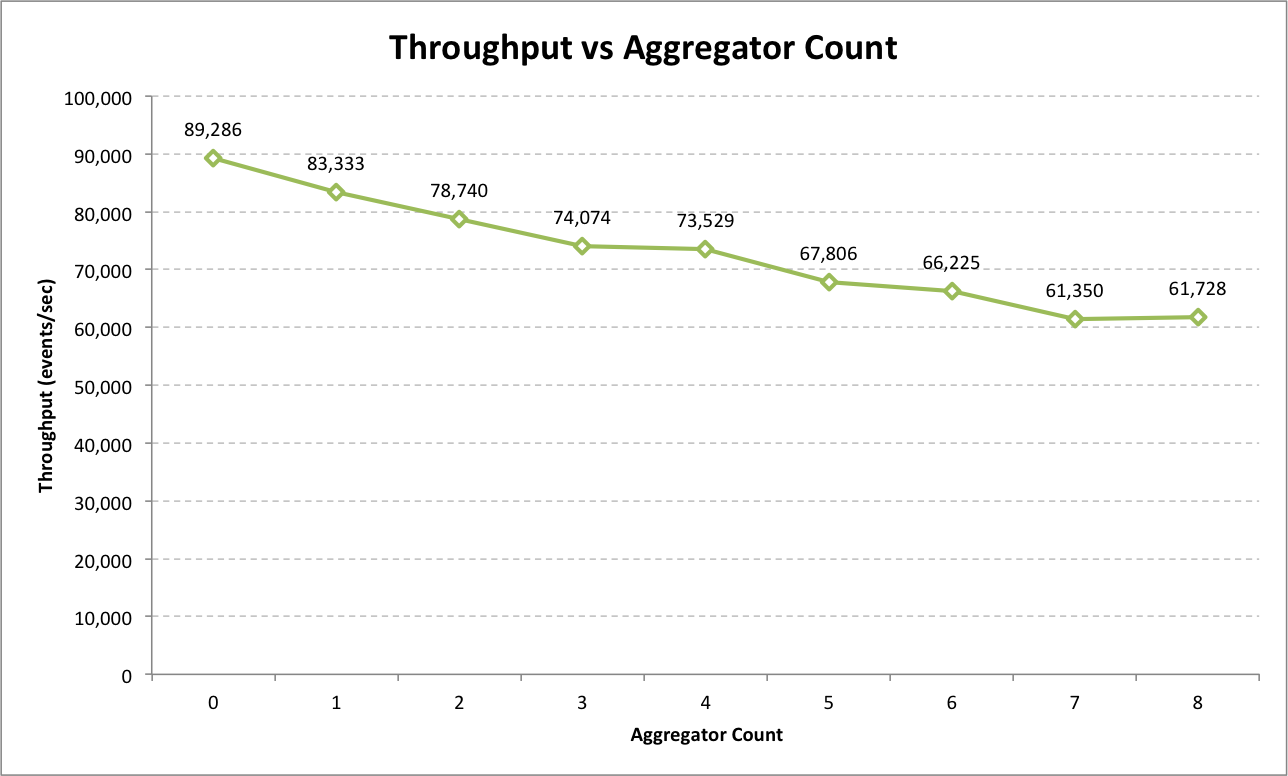
\includegraphics[width = 2.8in]{throughput_vs_num_metrics}
\caption{Adding new metrics to a data set decreases ingestion latency. In most
real world data sets, the number of metrics in a data set tends to be lower
than the number of dimensions.}
\label{fig:throughput_vs_num_metrics}
\end{figure}

\section{Related Work}
\label{sec:related}
Cattell \cite{cattell2011scalable} maintains a great summary about existing
Scalable SQL and NoSQL data stores. Hu \cite{hu2011stream} contributed another
great summary for streaming databases.  Druid feature-wise sits somewhere
between Google’s Dremel \cite{melnik2010dremel} and PowerDrill
\cite{hall2012processing}. Druid has most of the features implemented in Dremel
(Dremel handles arbitrary nested data structures while Druid only allows for a
single level of array-based nesting) and many of the interesting compression
algorithms mentioned in PowerDrill.

Although Druid builds on many of the same principles as other distributed
columnar data stores \cite{fink2012distributed}, many of these data stores are
designed to be more generic key-value stores \cite{stonebraker2005c} and do not
support computation directly in the storage layer.  There are also other data
stores designed for some of the same of the data warehousing issues that Druid
is meant to solve. These systems include include in-memory databases such as
SAP’s HANA \cite{farber2012sap} and VoltDB \cite{voltdb2010voltdb}. These data
stores lack Druid's low latency ingestion characteristics. Druid also has
native analytical features baked in, similar to \cite{paraccel2013}, however,
Druid allows system wide rolling software updates with no downtime.  

Druid's low latency data ingestion features share some similarities with
Trident/Storm \cite{marz2013storm} and Streaming Spark
\cite{zaharia2012discretized}, however, both systems are focused on stream
processing whereas Druid is focused on ingestion and aggregation. Stream
processors are great complements to Druid as a means of pre-processing the data
before the data enters Druid.

There are a class of systems that specialize in queries on top of cluster
computing frameworks.  Shark \cite{engle2012shark} is such a system for queries
on top of Spark, and Cloudera's Impala \cite{cloudera2013} is another system
focused on optimizing query performance on top of HDFS. Druid historical nodes
download data locally and only work with native Druid indexes. We believe this
setup allows for faster query latencies.

Druid leverages a unique combination of algorithms in its
architecture. Although we believe no other data store has the same set
of functionality as Druid, some of Druid’s optimization techniques such as using
inverted indices to perform fast filters are also used in other data
stores \cite{macnicol2004sybase}.

\section{Conclusions}
\label{sec:conclusions}
In this paper, we presented Druid, a distributed, column-oriented, real-time
analytical data store. Druid is designed to power high performance applications
and is optimized for low query latencies. Druid supports streaming data
ingestion and is fault-tolerant. We discussed how Druid was able to
scan 27 billion rows in a second. We summarized key architecture aspects such
as the storage format, query language, and general execution. In the future, we
plan to cover the different algorithms we’ve developed for Druid and how other
systems may plug into Druid in greater detail.

\balance

\section{Acknowledgements}
\label{sec:acknowledgements}
Druid could not have been built without the help of many great engineers at
Metamarkets and in the community.  We want to thank everyone that has
contributed to the Druid codebase for their invaluable support. 

% The following two commands are all you need in the
% initial runs of your .tex file to
% produce the bibliography for the citations in your paper.
\bibliographystyle{abbrv}
\bibliography{druid}  % druid.bib is the name of the Bibliography in this case
% You must have a proper ".bib" file
%  and remember to run:
% latex bibtex latex latex
% to resolve all references

%Generated by bibtex from your ~.bib file.  Run latex,
%then bibtex, then latex twice (to resolve references).

%APPENDIX is optional.
% ****************** APPENDIX **************************************
% Example of an appendix; typically would start on a new page
%pagebreak

\end{document}
